\documentclass[a4paper,12pt]{article}
\usepackage[utf8]{inputenc}
\usepackage[spanish]{babel}
\usepackage{color}
\usepackage{parskip}
\usepackage{graphicx}
\usepackage{multirow}
\usepackage{listings}
\usepackage{vmargin}
\usepackage{datetime}
\newdate{date}{13}{10}{2017}
\graphicspath{ {imagenes/} }
\definecolor{mygreen}{rgb}{0,0.6,0}
\definecolor{lbcolor}{rgb}{0.9,0.9,0.9}
\usepackage{epstopdf}
\usepackage{float}


\setpapersize{A4}
\setmargins{2.5cm}       % margen izquierdo
{1.5cm}                        % margen superior
{16.5cm}                      % anchura del texto
{23.42cm}                    % altura del texto
{10pt}                           % altura de los encabezados
{1cm}                           % espacio entre el texto y los encabezados
{0pt}                             % altura del pie de página
{2cm}     

\lstset{
%backgroundcolor=\color{lbcolor},
    tabsize=4,    
%   rulecolor=,
    language=[GNU]C++,
        basicstyle=\tiny,
        aboveskip={1.5\baselineskip},
        columns=fixed,
        showstringspaces=false,
        extendedchars=false,
        breaklines=true,
        prebreak = \raisebox{0ex}[0ex][0ex]{\ensuremath{\hookleftarrow}},
        frame=single,
        showtabs=false,
        showspaces=false,
        showstringspaces=false,
        identifierstyle=\ttfamily,
        keywordstyle=\color[rgb]{0,0,1},
        commentstyle=\color[rgb]{0.026,0.112,0.095},
        stringstyle=\color{red},
        numberstyle=\color[rgb]{0.205, 0.142, 0.73},
%        \lstdefinestyle{C++}{language=C++,style=numbers}’.
}


\begin{document}
\title{Ejercicios del libro}
\author{
Christofer Fabián Chávez Carazas \\
\small{Universidad Nacional de San Agustín de Arequipa} \\
\small{Escuela Profesional de Ciencia de la Computación} \\
\small{Computación Centrada en Redes}
}
\date{\displaydate{date}}

\maketitle

\begin{enumerate}
 \item \textbf{Imagine que entrenó a Bernie, su perro San Bernardo, para que transporte una caja de tres cintas de 8 mm
en vez de un termo con brandy (cuando se llene su disco, puede considerarlo una emergencia). Cada una de
estas cintas contiene 7 gigabytes. El perro puede viajar a donde quiera que vaya, a una velocidad de 18 km/h.
¿Para qué rango de distancias tiene Bernie una velocidad mayor de datos que una línea de transmisión cuya
velocidad de datos (sin sobrecarga) es de 150 Mbps? ¿Cómo cambiaría su respuesta si (i) se duplica la velocidad
de Bernie; (ii) se duplica la capacidad de cada cinta; (iii) se duplica la velocidad de datos de la línea
de transmisión?}

\begin{itemize}
 \item Bernie puede cargar 21 gigas de información. Haciendo la conversión, Bernie puede transportar 21,504 megas o 172,032 megabits.
  Para que la línea de transmisión pueda transportar todos esos datos se necesitan $172,032 / 150 = 1146.88$ segundos.
  La distancia que Bernie puede recorrer en 1,146.88 segundos es $1146.88 * 5 = 5734.4$ metros o 5.7 kilómetros. Entonces, Berinie
  tiene una velocidad mayor cuando la distancia de transmisión es menor a 5.7 kilómetros.
 \item Si se duplica la velocidad de Bernie, entonces su distancia que podría recorrer en 11,46.88 segundos seŕia $11,46.88 * 10 = 11,468.8$ metros o 11.5 kilómetros.
  Entonces, Bernie tiene una velocidad mayor cuando la distancia de transmisión es menor a 11.5 kilómetros.
 \item Si Bernie puede cargar 42 gigas de informacion, entonces puede transportar 344,064 megabits. Para que la línea de transmisión pueda transportar todos esos datos
  se necesitan $344,064 / 150 = 2,293.76$ segundos. La distancia que Bernie puede recorrer en 2,293.76 segundos es $2293.76 * 5 = 11,468.8$ metros o 11.5 kilómetros.
  Entonces, Bernie tiene una velocidad mayor cuando la distancia de transmisión es menor a 11.5 kilómetros.
 \item Si la velocidad de la línea es de 300 Mbps, entonces para que ésta pueda transportar todos los datos se necesitan $172,032/ 150 = 573.44$ segundos.
  La distancia que Bernie puede recorrer en 573.44 segundos es $573.44 * 5 = 2,867.2$ metros o 2.9 kilómetros.
  Entonces, Bernie tiene una  velocidad mayor cuando la distancia de transmisión es menor a 2.9 kilómetros.
\end{itemize}

 \item \textbf{El rendimiento de un sistema cliente-servidor se ve muy influenciado por dos características principales de las
redes: el ancho de banda de la red (es decir, cuántos bits/segundo puede transportar) y la latencia (cuántos segundos
tarda el primer bit en viajar del cliente al servidor). Cite un ejemplo de una red que cuente con un ancho
de banda alto pero también alta latencia. Después mencione un ejemplo de una red que tenga un ancho de banda
bajo y una baja latencia.}

\begin{itemize}
 \item Una de las redes más rápidas que deben existir son las conexiones transcontinentales, ya que, por lo que tienen que hacer, tienen un gran ancho de banda, y porque son
 conexiones de fibra óptica tienen una alta latencia.
 \item Una conexión bluetooth, por su naturaleza y en comparación, tiene poco ancho de banda y una baja latencia.
\end{itemize}

 \item \textbf{Un factor en el retardo de un sistema de conmutación de paquetes de almacenamiento y envío es cuánto tiempo
se requiere para almacenar y enviar un paquete a través de un switch. Si el tiempo de conmutación es de
10 microsegundos, ¿es probable que sea un factor importante en la respuesta de un sistema cliente-servidor en donde el
cliente está en Nueva York y el servidor en California? Asuma que la velocidad de propagación en cobre y fibra
óptica es de 2/3 la velocidad de la luz en el vacío.}

La velocidad de la luz es 299,792,458 m/s. La velocidad de propagación es 199,861,638 m/s que son 199,861638 metros por microsegundo; 200 redondeando.
La distancia entre Nueva York y California es de 4,694.3 kilómetros o 469,4300 metros. Entonces, se demoraría $469,4300 / 200 = 23471.5$ microsegundos.
Si hay 50 switches en el camino (una cantidad alta) el tiempo de conmutación sería 500 microsegundos, que vendría a ser el 2 porciento del total. Viendo esto se
podría decir que no es un factor importante.

 \item \textbf{En el futuro, cuando todos tengan una terminal casera conectada a una red de computadoras, serán posibles
los consultas públicas instantáneas sobre asuntos legislativos pendientes. En algún momento las legislaturas
existentes se podrían eliminar para dejar que el deseo del pueblo se exprese de manera directa. Los aspectos
positivos de tal democracia directa son bastante obvios; comente sobre algunos de los aspectos negativos}

Se podrían ver varios aspectos negativos en el aspecto político y social. También se podrían encontrar problemas
de seguridad en la red, por ejemplo, un hacker, teniendo un acceso más fácil, podría cambiar o insertar algunas
legislaciones.

 \item \textbf{Una desventaja de una subred de difusión es la capacidad que se desperdicia cuando varios hosts tratan de acceder
al canal al mismo tiempo. Como ejemplo simplista, suponga que el tiempo se divide en porciones (ranuras)
discretas y que cada uno de los n hosts trata de usar el canal con una probabilidad de p durante cada porción de
tiempo. ¿Qué fracción de las porciones se desperdiciará debido a las colisiones?}

Debido a que tiene un solo canal de comunicación compartido por todas las máquinas de la red, provoca la existencia de colisiones y el tiempo perdido sería relativamente poco ya que los mensajes cuentan con un campo de dirección dentro del paquete, el cual especifica a quien va dirigido y al recibir el paquete la máquina verifica el campo de dirección y si es dirigida a esta lo procesa y si no lo ignora, al perderse el paquete se pide una retransmisión para que este llegue a su destino.


 \item \textbf{A la presidenta de la empresa Specialty Paint Corp. se le ocurre la idea de trabajar con un fabricante de cerveza
local para producir una lata de cerveza invisible (como medida para reducir la basura). La presidenta ordena
a los de su departamento legal que investiguen el asunto; ellos a su vez piden ayuda al departamento de ingeniería.
Como resultado, el ingeniero en jefe llama a su homólogo en la compañía de cerveza para discutir los
aspectos técnicos del proyecto. Después los ingenieros se reportan con sus respectivos departamentos legales,
quienes entonces conversan por teléfono para arreglar los aspectos legales. Por último, los dos presidentes
corporativos discuten la cuestión financiera del trato. ¿Qué principio de un protocolo multicapas viola este
mecanismo de comunicación, en el sentido del modelo OSI?}

Uno de los principios del protocolo multicapas indica que las comunciaciones entre capas
es virtual y no física, siendo esta comunicación virtual estructurada a través de las capas del modelo
En este caso, los presidentes deberían comunicarse virtualmente a través de sus capas, o abogados e ingenieros, pero
los presidentes se comunican físicamente por teléfono, ignorando las capas y violando dicho principio.

 \item \textbf{¿Qué significa ``negociación'' al hablar sobre protocolos de red? Cite un ejemplo.}
 
La negociación es obtener en ambos lados un tipo de conveniencia con ciertos parámetros o valores que serán utilizados
durante la comunicación del servicio solicitado. Por ejemplo, podrían negociar el tamaño de los mensajes o la estructura de
éstos.

 \item \textbf{En algunas redes, la capa de enlace de datos se encarga los errores de transmisión pidiendo que se retransmitan
las tramas dañadas. Si la probabilidad de que una trama se dañe es p, ¿cuál es la cantidad promedio de transmisiones
requeridas para enviar una trama? Suponga que las confirmaciones de recepción nunca se pierden}

Si P es la probabilidad y N es el número de acuses entonces el promedio es: Promedio = P x N

 \item \textbf{¿Cuál es la principal diferencia entre TCP y UDP?}
 
 El protocolo TCP está orientado a la conexión, mediante el control de CRC, que verifica integridad de los datos,
 siendo un servicio más confiable. Si los datos son corruptos, se vuelven a solicitar. UDP es un protocolo no orientado a la conexión, ya que no se
 verifica la integridad de los datos, siendo un servicio menos confiable. Sin embargo su uso es grande en sistemas de streaming de videos.
 
 \item \textbf{Internet duplica su tamaño aproximadamente cada 18 meses. Aunque en realidad nadie lo sabe con certeza,
alguien estimó que el número de hosts que incluía era de 600 millones en 2009. Use estos datos para calcular el
número esperado de hosts de Internet para 2018. ¿Cree usted esto? Explique por qué si o por qué no.}

\begin{itemize}
 \item \textbf{2009:} 600 millones.
 \item \textbf{2012:} 2,400 millones.
 \item \textbf{2015:} 9,600 millones.
 \item \textbf{2018:} 38,400 millones.
\end{itemize}

Si es muy posible. Actualmente cada persona puede tener varios host conectados a internet gracias a la tecnología móvil e inalámbrica.
La tecnología va avanzando y cada vez más dispositivos que antes no se conectaban a internet ahora lo hacen. Como por ejemplo, televisores, refrigeradoras,
sensores, casas en su totalidad, generando así el concepto de internet de las cosas.

 \item \textbf{Los operadores de redes de telefonía móvil necesitan saber en dónde se encuentran los teléfonos móviles (y
sus usuarios). Explique por qué esto es malo para los usuarios. Ahora mencione las razones por las que esto es
bueno para los usuarios.}

Puede ser malo para los usuarios porque puede ser considerado una violación de la privacidad, y las ubicaciones pueden ser usadas por un hacker.
Una de las razones por la que esto podría ser bueno para los usuarios es que pueden localizar fácilmente su teléfono. Cuando su celular es hurtado, el usuario
puede localizar al ladrón o apagar su celular a distancia.

 \item \textbf{Una imagen tiene $1,600 x 1,200$ píxeles con 3 bytes/píxel. Suponga que no está comprimida. ¿Cuánto tiempo
tarda en transmitirse a través de un canal de modem de 56 kbps? ¿A través de un módem de cable de 1 Mbps?
¿A través de una red Ethernet de 10 Mbps? ¿A través de una red Ethernet de 100 Mbps? ¿A través de una red
Gigabit Ethernet de 1 Gbps?}
 
En total tenemos 5,760,000 bytes que tienen que ser transportados.
 
\begin{itemize}
 \item Con el módem de 56 kbps: Tienen que ser transportados 5,625 KB o 45,000 Kb. El tiempo que demora es $45,000 / 56 = 803.57$ segundos.
 \item Con el módem de 1 Mbps: 	Tienen que ser transportados 5.4932 MB o 43.945 Mb. El tiempo que demora es $43.945 / 1 = 43.945$ segundos.
 \item Con una red Ethernet de 10 Mbps: Tienen que ser transportados 5.4932 MB o 43.945 Mb. El tiempo que demora es $43.945 / 10 = 4.3945$ segundos.
 \item Con una red Ethernet de 100 Mbps: Tienen que ser transportados 5.4932 MB o 43.945 Mb. El tiempo que demora es $43.945 / 100 = 0.43945$ segundos.
 \item Con una red Gigabit Ethernet de 1 Gbps: Tienen que ser transportados 0.0053644 o GB o 0.042915 Gb. El tiempo que demora es $0.042915 / 1 = 0.042915$ segundos.
\end{itemize}

 \item \textbf{Mencione dos ventajas y dos desventajas de tener estándares internacionales para los protocolos de red}
 
 Una de las principales ventajas es que al crear nuevos productos simplemente se utilizan dichos protocolos y esto genera una buena compatibilidad entre dispositivos. La segunda ventaja
 es la facilidad de intercambiar información sin errores de comunicación. Una desventaja es que los protocolos tienen sus límites. Y otra desventaja es que, al ser los protocolos
 públicos y muy conocidos, los hackers la tienen fácil al momento de intentar sus ataques.
 
 \item \textbf{Suponga que se cambian los algoritmos utilizados para implementar las operaciones en la capa k. ¿Cómo puede
afectar esto a las operaciones en las capas $k - 1$ y $k + 1$?}

 En la capa $k-1$ puede afectar cuando se recibe la respuesta de la capa superior y en la capa $k+1$ puede afectar el tamaño en bytes, formato y el significado del paquete.
 
 \item \textbf{Proporcione una lista de razones por las que el tiempo de respuesta de un cliente puede ser mayor que el retardo
en el mejor de los casos.}

\begin{itemize}
 \item Porque puede ser que se pueda estancar en algunas de las rutas.
 \item Que el paquete no cumpla con los protocolos establecidos.
 \item Puede ser que por la ruta por donde va ser enviado el paquete no esté en funcionamiento, por lo que tendrá que buscar otra ruta.
\end{itemize}

 \item \textbf{Haga una lista de actividades que realiza a diario en donde se utilicen redes de computadoras. ¿Cómo se alteraría
su vida si de repente se apagaran estas redes?}

\begin{itemize}
 \item Cuando hago tareas grupales.
 \item En reuniones remotas.
 \item En el laboratorio de la universidad.
 \item En las clases al hacer anotaciones.
 \item Cada vez que me comunico por cualquier aplicación de mensajería.
 \item Al jugar videojuegos.
\end{itemize}

Se podría decir que todo sería más difícil de realizar. Por ejemplo, para hacer las tareas grupales tendríamos que reunirnos físicamente.

 \item \textbf{El programa ping le permite enviar un paquete de prueba a una ubicación dada para ver cuánto tarda en llegar
hasta allá y regresar. Pruebe a usar ping para ver cuánto tiempo se requiere para ir de su ubicación hasta varias
ubicaciones conocidas. Con base en estos datos, trace el tiempo de tránsito de una sola dirección a través de
Internet en función de la distancia. Lo más adecuado es utilizar universidades, ya que la ubicación de sus servidores
se conoce con mucha precisión. Por ejemplo, berkeley.edu está en Berkeley, California; mit.edu está en
Cambridge, Massachusetts; vu.nl está en Amsterdam, Holanda; www.usyd.edu.au está en Sydney, Australia; y
www.uct.ac.za está en Cape Town, Sudáfrica}

\begin{itemize}
 \item Berkeley, California: 173 ms
 \item Cambridge, Massachusetts: 64.3 ms
 \item Amsterdam, Holanda: 225 ms
 \item Sydney, Australia: 327 ms
 \item Cape Town, Sudáfrica: No hay respuesta.
\end{itemize}

 \item \textbf{Internet está compuesta de una gran cantidad de redes. Su arreglo determina la topología de Internet. Hay
una cantidad considerable de información en línea sobre la topología de Internet. Use un motor de búsqueda
para averiguar más sobre la topología de Internet y escriba un breve informe con una síntesis de sus
hallazgos.}

La topología de Internet es la fuente básica del poder en la Red (Servidores Raíz, clases de IP, asignación de los mismos). Al contrario que el territorio real, cuya existencia es previa a la persona, el nuevo territorio responde a un diseño de la misma.
La topología de internet es un conjunto de redes al alcance de todos, ya que está surgiendo movimientos nuevos a favor de otro tipo de la red de redes movimientos, tales como
el de Free Network Project que han diseñado un sistema de servidores y clientes en los que se busca el más absoluto anónimo de la Red. Para ello debe modificarse el uso del topológico actual, por lo que se prescinde de los servidores raíz y la asignación de DNS.

 \item \textbf{Escriba un programa que implemente el flujo de mensajes desde la capa más alta hasta la capa más baja del
modelo de protocolos de siete capas. Su programa debe incluir una función de protocolo separada para cada
capa. Los encabezados de los protocolos son secuencias de hasta 64 caracteres. Cada función de protocolo tiene
dos parámetros: un mensaje que se pasa del protocolo de la capa superior (un búfer de caracteres) y el tamaño
del mensaje. Esta función añade su encabezado al frente del mensaje, imprime el nuevo mensaje en la salida
estándar y después invoca a la función de protocolo del protocolo de la capa inferior. La entrada del programa es
un mensaje de aplicación (una secuencia de 80 caracteres o menos)}

\begin{lstlisting}
#include <iostream>

using namespace std;

void protocolo7(string mensaje){
	cout<<"Protocolo 7: "<<mensaje<<endl;
	cout<<"Mensaje enviado"<<endl;
}

void protocolo6(string mensaje){
	cout<<"Protocolo 6: "<<mensaje<<endl;
	protocolo7(mensaje);
}

void protocolo5(string mensaje){
	cout<<"Protocolo 5: "<<mensaje<<endl;
	protocolo6(mensaje);
}

void protocolo4(string mensaje){
	cout<<"Protocolo 4: "<<mensaje<<endl;
	protocolo5(mensaje);
}

void protocolo3(string mensaje){
	cout<<"Protocolo 3: "<<mensaje<<endl;
	protocolo4(mensaje);
}

void protocolo2(string mensaje){
	cout<<"Protocolo 2: "<<mensaje<<endl;
	protocolo3(mensaje);
}

void protocolo1(string mensaje){
	cout<<"Protocolo 1: "<<mensaje<<endl;
	protocolo2(mensaje);
}

int main(int argc, char const ** argv){
	if(argc != 2){
		cout<<"Faltan argumentos <mensaje>"<<endl;
		return 0;
	}
	string mensaje(argv[1]);
	protocolo1(mensaje);
	return 0;
}
\end{lstlisting}

\textbf{Resultados:} \\
\begin{figure}[H]
 \centering
 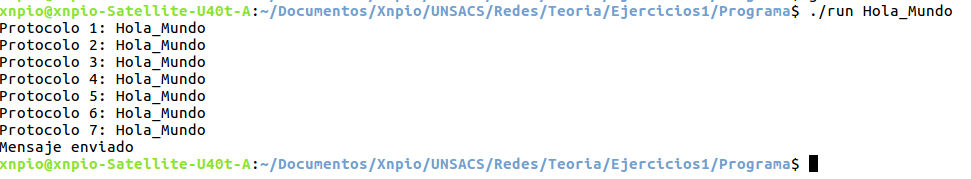
\includegraphics[scale = 0.5]{1.png}
\end{figure}




 
 
 
\end{enumerate}



\end{document}

